\documentclass[a4paper, final]{article}
\usepackage{cmap}
%\usepackage{literat} % Нормальные шрифты
\usepackage[14pt]{extsizes} % для того чтобы задать нестандартный 14-ый размер шрифта
\usepackage[T2A]{fontenc}
\usepackage[UTF8]{inputenc}
\usepackage[russian]{babel}
\usepackage{listings} %листинги
\usepackage{amsmath}
\usepackage{amssymb} % Для красивого значка пустого множества
\usepackage[left=25mm, top=20mm, right=20mm, bottom=20mm, footskip=10mm]{geometry}
\usepackage{ragged2e} %для растягивания по ширине
\usepackage{setspace} %для межстрочного интервала
\usepackage{indentfirst} % для абзацного отступа
\usepackage{moreverb} %для печати в листинге исходного кода программ
\renewcommand\verbatimtabsize{4\relax}
\renewcommand\listingoffset{0.2em} %отступ от номеров строк в листинге
\renewcommand{\arraystretch}{1.4} % изменяю высоту строки в таблице
\usepackage[font=small, singlelinecheck=false, justification=centering, format=plain, labelsep=period]{caption} %для настройки заголовка таблицы
\usepackage{listingsutf8}
\usepackage{xcolor} % цвета
\usepackage{hyperref}% для гиперссылок
\usepackage{enumitem} %для перечислений
\usepackage{titlesec}
\usepackage{graphicx}
\graphicspath{ {./Рисунки/} }
%\usepackage{float}
\usepackage{booktabs}
\usepackage{floatrow}
\usepackage{scalerel} % Stretching images
\usepackage[final]{pdfpages}
\usepackage{multirow}
\usepackage{array}
\usepackage{tabularx}

\definecolor{apricot}{HTML}{FFF0DA}
\definecolor{mygreen}{rgb}{0,0.6,0}
\definecolor{string}{HTML}{B40000} % цвет строк в коде
\definecolor{comment}{HTML}{008000} % цвет комментариев в коде
\definecolor{keyword}{HTML}{1A00FF} % цвет ключевых слов в коде
\definecolor{morecomment}{HTML}{8000FF} % цвет include и других элементов в коде
\definecolor{captiontext}{HTML}{FFFFFF} % цвет текста заголовка в коде
\definecolor{captionbk}{HTML}{999999} % цвет фона заголовка в коде
\definecolor{bk}{HTML}{FFFFFF} % цвет фона в коде
\definecolor{frame}{HTML}{999999} % цвет рамки в коде
\definecolor{brackets}{HTML}{B40000} % цвет скобок в коде





\AtBeginDocument{\renewcommand{\contentsname}{Содержание}}
\AtBeginDocument{\renewcommand{\refname}{Список источников}}
% Настраиваем листинги, чтобы они использовали счётчик figure
\AtBeginDocument{
  \renewcommand{\thelstlisting}{\thefigure}  % Листинги используют тот же счетчик, что и рисунки
  \renewcommand{\lstlistingname}{Рис.}    % Меняем подпись
}

% Автоматически увеличиваем счетчик figure перед каждым листингом
\let\oldlstlisting\lstlisting
\renewcommand{\lstlisting}[1][]{%
    \refstepcounter{figure}% Увеличиваем счетчик figure
    \oldlstlisting[#1]% Вызываем оригинальную команду lstlisting
}
\lstset{
    captionpos=b
}
\newcommand{\specialcell}[2][l]{\begin{tabular}[#1]{@{}l@{}}#2\end{tabular}} % Алиас для таблиц

\floatsetup[table]{style=plain,capposition=top} % Подпись таблицы сверху
\setlist[enumerate,itemize]{leftmargin=1.2cm} %отступ в перечислениях

\hypersetup{colorlinks,
  allcolors=[RGB]{000 000 000}} %красивые гиперссылки (не красные)

% подгружаемые языки — подробнее в документации listings (это всё для листингов)
\lstloadlanguages{ [LaTeX] TeX}
% включаем кириллицу и добавляем кое−какие опции
\lstset{language =[LaTeX] TeX, % выбираем язык по умолчанию
extendedchars=true , % включаем не латиницу
escapechar = | , % |«выпадаем» в LATEX|
frame=tb , % рамка сверху и снизу
commentstyle=\itshape , % шрифт для комментариев
stringstyle =\bfseries} % шрифт для строк

\textheight=24cm % высота текста
\textwidth=16cm % ширина текста
\oddsidemargin=0pt % отступ от левого края
\topmargin=-1.5cm % отступ от верхнего края
\parindent=24pt % абзацный отступ
\parskip=0pt % интервал между абзацами
\tolerance=2000 % терпимость к "жидким" строкам
\flushbottom % выравнивание высоты страниц

\begin{document} % начало документа
\setcounter{tocdepth}{2} % Вложенность не больше 2 в содержании
\lstset{
  language=haskell, % Язык кода по умолчанию
  morekeywords={*,...}, % если хотите добавить ключевые слова, то добавляйте
  % Цвета
  keywordstyle=\color{keyword}\ttfamily\bfseries,
  %stringstyle=\color{string}\ttfamily,
  stringstyle=\ttfamily\color{red!50!brown},
  commentstyle=\color{comment}\ttfamily,
  morecomment=[l][\color{morecomment}]{\#},
  % Настройки отображения
  breaklines=true, % Перенос длинных строк
  basicstyle=\ttfamily\footnotesize, % Шрифт для отображения кода
  backgroundcolor=\color{bk}, % Цвет фона кода
  frame=single,xleftmargin=\fboxsep,xrightmargin=-\fboxsep, % Рамка, подогнанная к заголовку
  rulecolor=\color{frame}, % Цвет рамки
  tabsize=3, % Размер табуляции в пробелах
  % Настройка отображения номеров строк. Если не нужно, то удалите весь блок
  numbers=left, % Слева отображаются номера строк
  stepnumber=1, % Каждую строку нумеровать
  numbersep=5pt, % Отступ от кода
  numberstyle=\small\color{black}, % Стиль написания номеров строк
  % Для отображения русского языка
  extendedchars=true,
  literate={Ö}{ {\"O} }1
  {~}{ {\textasciitilde} }1
  {а}{ {\selectfont\char224} }1
  {б}{ {\selectfont\char225} }1
  {в}{ {\selectfont\char226} }1
  {г}{ {\selectfont\char227} }1
  {д}{ {\selectfont\char228} }1
  {е}{ {\selectfont\char229} }1
  {ё}{ {\"e} }1
  {ж}{ {\selectfont\char230} }1
  {з}{ {\selectfont\char231} }1
  {и}{ {\selectfont\char232} }1
  {й}{ {\selectfont\char233} }1
  {к}{ {\selectfont\char234} }1
  {л}{ {\selectfont\char235} }1
  {м}{ {\selectfont\char236} }1
  {н}{ {\selectfont\char237} }1
  {о}{ {\selectfont\char238} }1
  {п}{ {\selectfont\char239} }1
  {р}{ {\selectfont\char240} }1
  {с}{ {\selectfont\char241} }1
  {т}{ {\selectfont\char242} }1
  {у}{ {\selectfont\char243} }1
  {ф}{ {\selectfont\char244} }1
  {х}{ {\selectfont\char245} }1
  {ц}{ {\selectfont\char246} }1
  {ч}{ {\selectfont\char247} }1
  {ш}{ {\selectfont\char248} }1
  {щ}{ {\selectfont\char249} }1
  {ъ}{ {\selectfont\char250} }1
  {ы}{ {\selectfont\char251} }1
  {ь}{ {\selectfont\char252} }1
  {э}{ {\selectfont\char253} }1
  {ю}{ {\selectfont\char254} }1
  {я}{ {\selectfont\char255} }1
  {А}{ {\selectfont\char192} }1
  {Б}{ {\selectfont\char193} }1
  {В}{ {\selectfont\char194} }1
  {Г}{ {\selectfont\char195} }1
  {Д}{ {\selectfont\char196} }1
  {Е}{ {\selectfont\char197} }1
  {Ё}{ {\"E} }1
  {Ж}{ {\selectfont\char198} }1
  {З}{ {\selectfont\char199} }1
  {И}{ {\selectfont\char200} }1
  {Й}{ {\selectfont\char201} }1
  {К}{ {\selectfont\char202} }1
  {Л}{ {\selectfont\char203} }1
  {М}{ {\selectfont\char204} }1
  {Н}{ {\selectfont\char205} }1
  {О}{ {\selectfont\char206} }1
  {П}{ {\selectfont\char207} }1
  {Р}{ {\selectfont\char208} }1
  {С}{ {\selectfont\char209} }1
  {Т}{ {\selectfont\char210} }1
  {У}{ {\selectfont\char211} }1
  {Ф}{ {\selectfont\char212} }1
  {Х}{ {\selectfont\char213} }1
  {Ц}{ {\selectfont\char214} }1
  {Ч}{ {\selectfont\char215} }1
  {Ш}{ {\selectfont\char216} }1
  {Щ}{ {\selectfont\char217} }1
  {Ъ}{ {\selectfont\char218} }1
  {Ы}{ {\selectfont\char219} }1
  {Ь}{ {\selectfont\char220} }1
  {Э}{ {\selectfont\char221} }1
  {Ю}{ {\selectfont\char222} }1
  {Я}{ {\selectfont\char223} }1
  {\{}{ { {\color{brackets}\{} } }1 % Цвет скобок {
  {\} }{ { {\color{brackets}\} } } }1 % Цвет скобок }
}

% НАЧАЛО ТИТУЛЬНОГО ЛИСТА
\begin{center}
\hfill \break
\hfill \break
\normalsize{МИНИСТЕРСТВО НАУКИ И ВЫСШЕГО ОБРАЗОВАНИЯ РОССИЙСКОЙ ФЕДЕРАЦИИ\\
 федеральное государственное автономное образовательное учреждение высшего образования «Санкт-Петербургский политехнический университет Петра Великого»\\[5pt]}
\normalsize{Институт компьютерных наук и кибербезопасности}\\[5pt] 
\normalsize{Высшая школа технологий искусственного интеллекта}\\[5pt] 
\normalsize{Направление: 02.03.01 Математика и компьютерные науки}\\

\hfill \break
\hfill \break
\hfill \break
\large{\textbf{Технологии разработки ПО}}\\
\hfill \break
\large{<<Формальное описание процесса разработки модуля кодирования и декодирования графа кодом Прюфера с помощью методологии IDEF0>>}\\

\hfill \break
\hfill \break
\end{center}
 
\small{ 
\begin{tabular}{lrrl}
\!\!\!Студент, & \hspace{2cm} & & \\
\!\!\!группы 5130201/20102 & \hspace{2cm} & \underline{\hspace{3cm}} & Гаар В.С. \\\\
\!\!\!Преподаватель, \hspace{2cm} & & \\
\!\!\!к.т.н., доц. & \hspace{2cm} & \underline{\hspace{3cm}} &  Курочкин М.А. \\\\
&&\hspace{5cm}
\end{tabular}
\begin{flushright}
<<\underline{\hspace{1cm}}>>\underline{\hspace{2.5cm}} 2024 г.
\end{flushright}
}

\hfill \break
\hfill \break
\begin{center} \small{Санкт-Петербург, 2024} \end{center}
\thispagestyle{empty} % выключаем отображение номера для этой страницы

% КОНЕЦ ТИТУЛЬНОГО ЛИСТА
\newpage

\tableofcontents

\newpage

\cleardoublepage
\phantomsection
\addcontentsline{toc}{section}{Введение}
\section*{Введение}
Общая методология IDEF состоит из трех частных
методологий моделирования, основанных на графическом представлении
систем:
\begin{itemize}
  \item IDEF0 используется для создания функциональной модели, отображающей
  структуру и функции системы, а также потоки информации и материальных 
  объектов, связывающие эти функции.
  \item IDEF1 применяется для построения информационной модели, отображающей
  структуру и содержание информационных потоков, необходимых для 
  поддержки функций системы;
  \item IDEF2 позволяет построить динамическую модель меняющихся во времени
  поведения функций, информации и ресурсов системы.
\end{itemize}

В нашей работе используется методология IDEF0. Она позволяет исследовать функции организации, не связывая их с объектами, обеспечивающими их реализацию.

В данном случае объектом моделирования является процесс разработки модуля кодирования и декодирования графа 
кодом Прюфера.

\newpage
\section{Постановка задачи}
\noindent Для выполнения работы были поставлены следующие задачи:
\begin{enumerate}
	\item Изучить методологию IDEF0.
	\item В рамках этой методологии создать функциональную модель модуля кодирования и декодирования графа кодом Прюфера.
\end{enumerate}

\newpage
\section{Основные понятия методологии и языка IDEF0}
Основу методологии IDEF0 составляет графический язык описания процессов.

{\bf Графический язык} --- полное и выразительное средство, способное наглядно представлять широкий спектр деловых, 
производственных и других процессов и операций предприятия на любом уровне детализации.

Язык обеспечивает точное и лаконичное описание моделируемых объектов, удобство использования и интерпретации этого описания.

{\bf Модель} в нотации IDEF0 представляет собой совокупность иерархически упорядоченных и взаимосвязанных диаграмм. 
Каждая диаграмма является единицей описания системы и располагается на отдельном листе.

{\bf Контекст} --- окружающая среда, в которой действует функция (или комплект функций на диаграмме).

{\bf Контекстная диаграмма} --- диаграмма, имеющая узловой номер A-n $( n\ge 0 )$, которая представляет контекст модели.

{\bf Диаграмма A-0} --- специальный вид контекстной диаграммы IDEF0, состоящей из одного блока, описывающего функцию 
верхнего уровня, ее входы, выходы, управления, и механизмы, вместе с формулировками цели модели и точки зрения, 
с которой строится модель.

{\bf Декомпозиция} ---  разделение моделируемой функции на функции-компоненты.

{\bf Блоки} представляют основные функции моделируемого объекта. Эти функции могут быть разбиты (декомпозированы) 
на составные части и представлены в виде более подробных диаграмм. Процесс декомпозиции продолжается до тех пор, пока 
объект не будет описан на уровне детализации, необходимом для достижения целей конкретного проекта. 

{\bf Дочерняя диаграмма} --- диаграмма, создаваемая при декомпозиции, охватывающая ту же область, что и родительский блок, 
но описывающая ее более подробно.

Таким образом, единственная функция, представленная на контекстной диаграмме верхнего уровня А-0, 
может быть разложена на основные подфункции посредством создания дочерней диаграммы А0.

{\bf Базовые требования стандарта IDEF0:}
\begin{enumerate}
	\item В левом верхнем углу всегда -- главный элемент.
	\item Все элементы должны иметь входящие и исходящие стрелки, так как для выполнения необходимо что-то
	получить на входе (заказ, поставленную задачу), а после обработки на выходе необходимо передать готовый
	продукт. Входящие стрелки всегда слева, исходящие –- справа.
	\item Сверху – управляющие элементы, снизу –- механизмы, необходимые для выполнения процесса.
	\item Если на одном листе (экране) располагается несколько блоков, каждый последующий располагается справа
	и ниже предыдущего.
	\item Необходимо стремиться создавать схемы таким образом, чтобы пересечение стрелок 
	было сведено к необходимому минимуму. \cite{bib:gost_idef0}
\end{enumerate}

% \par Пример структуры IDEF0-модели представлен на рисунке №~\ref{img:struct}, где приведены четыре диаграммы и их 
% взаимосвязи.
% \newpage
% \begin{figure}[H]
% 	\centering
% 	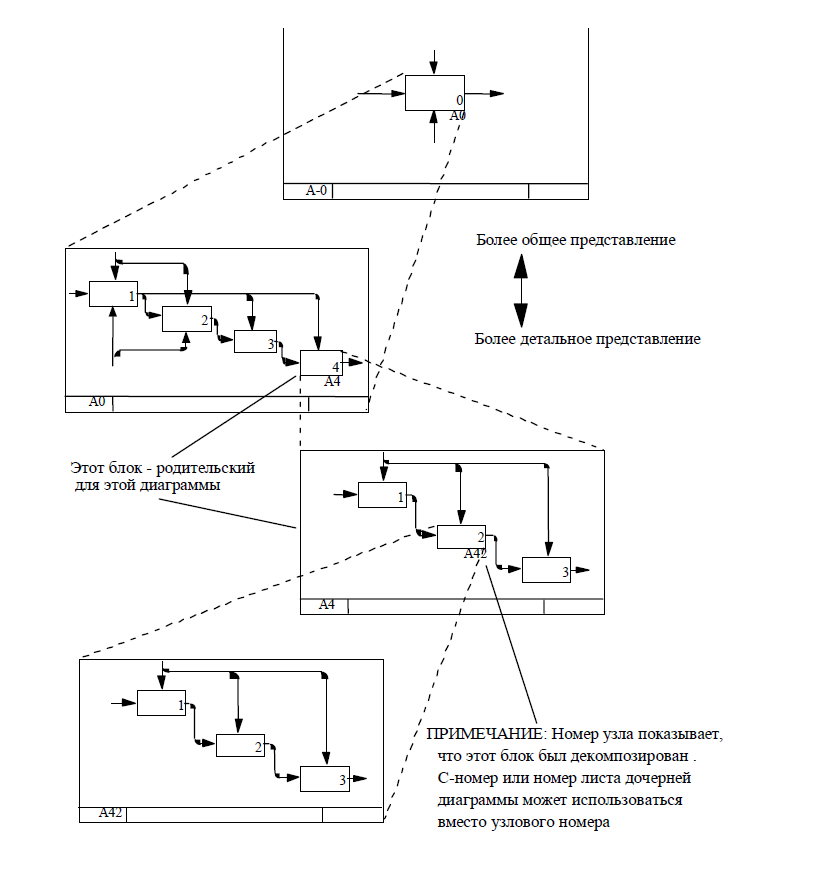
\includegraphics[scale = 0.7]{struct.png}
% 	\caption{Пример структуры IDEF0-модели}
% 	\label{img:struct}
% \end{figure}

\newpage
\section{Концепия IDEF0}
Методология IDEF0 основана на следующих концепциях:
\begin{enumerate}
	\item {\bfГрафическое и текстовое представление моделируемой деятельности.} \\
Графическая и текстовая нотация блочного моделирования в IDEF0-диаграм-мах показывает производственные операции 
(блок) и взаимосвязи с операциями (стрелки, входящие/покидающие блок). Наличие четко описанных нотаций обеспечивает 
корректность встроенных в иерархическую структуру модели диаграмм.

В IDEF0 все, что происходит в системе и ее элементах, принято называть {\bf функциями}. Каждой функции ставится в соответствие {\bf блок}. 
Для того чтобы представить реальные производственные операции, блоки могут быть интерпретированы как деятельность, связанная с другими блоками, 
с интерфейсными стрелками, определяющими, когда и как переключаются или управляются операции. Взаимодействие блоков друг с другом описываются 
посредством {\bf интерфейсных стрелок}, выражающих «ограничения», которые в свою очередь определяют, когда и каким образом функции выполняются и 
управляются.

	\item {\bf Компактность.} \\
Документация с описанием производственной архитектуры должна быть компактной для простого ориентирования в 
предмете. Двухмерная форма, описанная на языке диаграмм, достигает компактности без потери возможности выражения 
отношений, таких как интерфейсы и обратная связь. IDEF0-диаграммы позволяют представить любую изучаемую и/или 
описываемую систему в виде обеспечивающей компактность информации иерархии взаимодействующих и взаимосвязанных 
блоков, отображающих процессы, операции, действия.

	\item {\bf Функциональная декомпозиция.} \\
Одной из наиболее важных особенностей методологии IDEF0 является постепенное введение все больших 
уровней детализации по мере создания диаграмм, отображающих модель.

{\it Функциональная декомпозиция} --- способ моделирования ситуации, когда любое действие, операция, 
функция могут быть декомпозированы на более простые действия, операции, функции. Другими словами, сложный 
процесс может быть представлен в виде совокупности элементарных функций. Представляя функции графически, в 
виде блоков, можно заглянуть внутрь блока и детально рассмотреть его структуру.

	\item {\bf Обмен информацией.} \\
Диаграммы IDEF0 базируются на простой графике, состоящей из блоков и стрелок, легко читаемы и понимаемы. 
Средства IDEF0 облегчают передачу информации от одного участника разработки модели (разработчика или рабочей
группы) к другому. К числу таких средств относятся:
\begin{itemize}
\item метки на естественном языке для описания блоков и стрелок, а также глоссарий и сопроводительный текст для точного 
определения понятий элементов диаграммы;
\item последовательная декомпозиция диаграмм модели, использование иерархии с главной функцией на верху модели и 
дальнейшее разбитие на подфункции при углублении вниз;
\item древовидные схемы иерархии диаграмм и блоков, обеспечивающие обозримость модели в целом и входящих в нее деталей;
\item индексирование диаграмм и блоков, позволяющее однозначно обращаться к ним в ие рархической структуре модели;
\item ограничения (не более 6 блоков на диаграмму) введены для простого восприятия диаграмм.
\end{itemize}

	\item {\bf Строгость, точность, формализм и однозначность.} \\
Разработка моделей IDEF0 требует соблюдения ряда строгих формальных правил, обеспечивающих преимущества методологии 
в отношении однозначности, точности и целостности сложных многоуровневых моделей. Качество модели обеспечивается 
соблюдением следующих требований:
\begin{itemize}
\item Все стадии и этапы разработки и корректировки модели должны строго, формально документироваться с тем, чтобы при 
ее эксплуатации не возникало вопросов, связанных с неполнотой или некорректностью документации;
\item Разделение входов и управлений (правило определения роли данных);
\item Обязательное наличие управления (все блоки требуют как минимум одного управляющего входа) ;
\item Подробное описание на каждом уровне (3-6 блоков).
\item Ограниченный контекст (только то, что относится к делу и ничего лишнего, ничего не упущено).
\item Требования к меткам дуг данных (правила минимальных меток). 
\end{itemize}

	\item {\bf Итеративное моделирование.} \\
Разработка модели в IDEF0 представляет собой пошаговую, итеративную процедуру. На каждом шаге итерации разработчик 
предлагает вариант модели, который подвергают обсуждению, рецензированию и последующему редактированию, после чего 
цикл повторяется. 

Такая организация работы способствует оптимальному использованию знаний системного аналитика, владеющего методологией 
и техникой IDEF0, и знаний специалистов – экспертов в предметной области, к которой относится объект моделирования.

	\item {\bf Отделение <<организации>> от <<функций>>.} \\
Отделение организации от функции включено в цель модели и осуществляется отбором имен функций и связей в процессе 
разработки модели. При разработке моделей следует избегать изначальной «привязки» функций исследуемой системы к 
существующей организационной структуре моделируемого объекта (предприятия, фирмы). 
\par Это помогает избежать субъективной точки зрения, навязанной организацией и ее руководством. Организационная 
структура должна явиться результатом применения модели. \cite{bib:gost2_idef0}
\end{enumerate}

\newpage
\section{Модель IDEF0}
% {\bf Модель IDEF0} --- графическое описание системы, разработанное с определенной целью и с выбранной точки зрения. 
% Комплект одной или более диаграмм IDEF0, которые изображают функции системы с помощью графики, текста и глоссария.


\subsection{Контекстная диаграмма А-0}

Моделирование процесса начинается именно с построения контекстной диаграммы. Эта диаграмма с единственным блоком определяет
контекст всей модели и образует основу для дальнейшей декомпозиции. 
\par На Рис. 1 педставлена диаграмма А-0. Контекстная диаграмма устанавливает область моделирования и границу 
области моделирования. Данная диаграмма задает основные параметры процесса разработки модуля кодирования и декодирования графа
кодом Прюфера с точки зрения разработчика-программиста. 

\par {\bf Входные данные:} техническое задание.

\par {\bf Выходные данные:} разработанный модуль кодирования и декодирования графа кодом Прюфера.

\par {\bf Управляющие данные:} нормативные документы.

\par {\bf Механизмы:} программист, язык программирования С++ и среда разработки Visual Studio 2022. 

\newpage
\hypertarget{img:A-0}{}
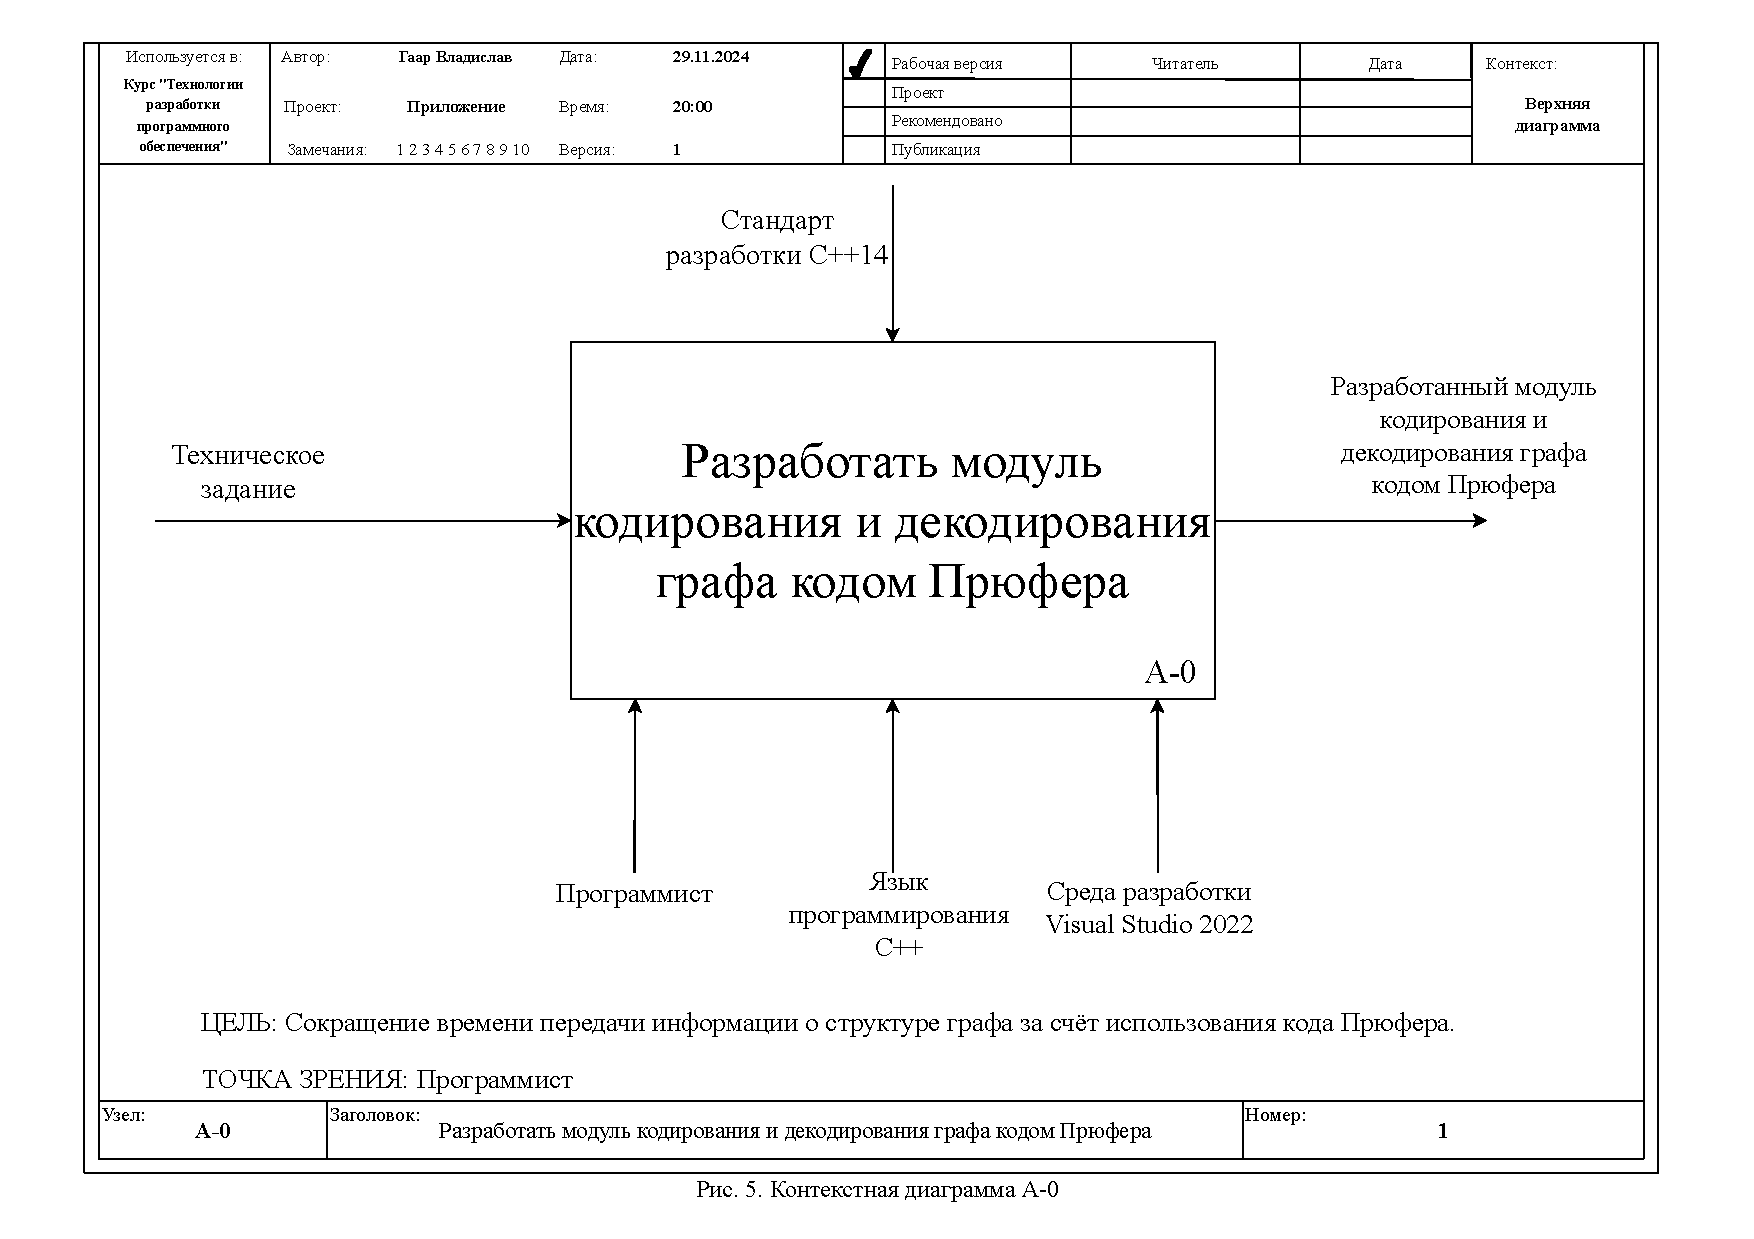
\includepdf[pages=1, fitpaper]{A-0.pdf}


\subsection{Диаграммы декомпозиций}
\subsubsection{Диаграмма А0}

На Рис. 2 представлена дочерняя диаграмма А0. Данная диаграмма представляет собой декомпозицию общего блока на 
элементы, которые связаны между собой.

Были выделены следующие блоки:

\begin{itemize}
	\item[A1.] Реализовать функции ввода данных и выбора способа задания графа;
	\item[A2.] Реализовать функцию генерации графа;
	\item[A3.] Реализовать функцию кодирования графа кодом Прюфера;
	\item[A4.] Реализовать функцию декодирования графа из кодов Прюфера;
	\item[A5.] Объединить реализованные функции.
\end{itemize} 

Управляющим воздействием всех блоков являются нормативные документы, механизмами являются язык программирования С++ 
и среда разработки Visual Studio 2022.

На вход блокам подается техническое задание на модуль кодирования и декодирования графа кодом Прюфера. На каждый 
блок поступают конкретные требования из технического задания, необходимые для разработки конкретных функций системы.

На выходе блоков получаются разработанные функции для работы с вводом данных, генерации графа, кодирования и декодирования
графа кодом Прюфера.

Стрелки, входящие в блок и выходящие из него на диаграмме верхнего уровня, являются теми же самыми, что и стрелки, 
входящие в диаграмму нижнего уровня и выходящие из нее, потому что блок и диаграмма представляют одну и ту же 
часть системы. Как следствие этого, границы функции верхнего уровня 
-- это то же самое, что и границы диаграммы декомпозиции.

\newpage
\hypertarget{img:A0}{}
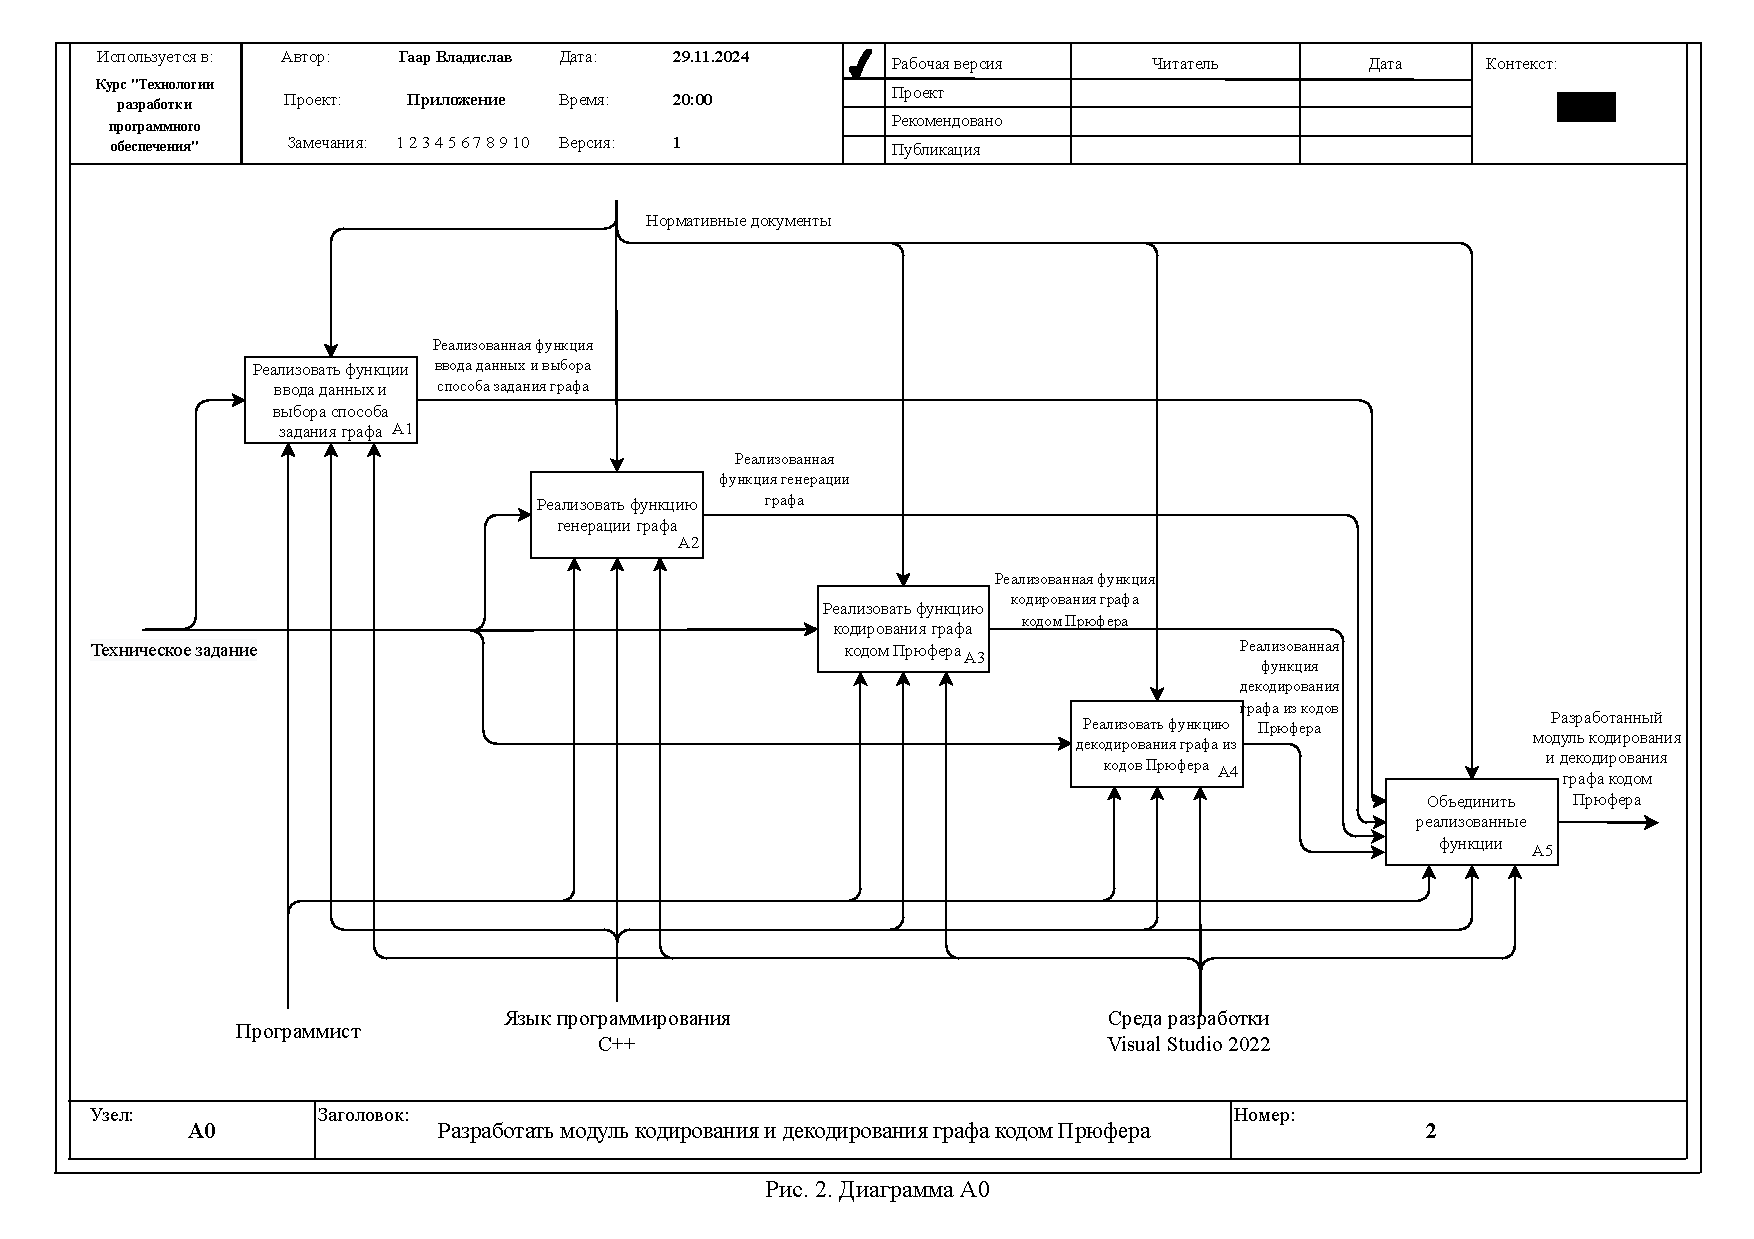
\includepdf[pages=1, fitpaper]{A0.pdf}


\subsubsection{Диаграмма А1}
Блок <<Реализовать функции ввода данных и выбора способа задания графа>> дочерней диаграммы А0 (см. Рис. \ref{img:A0}) может 
быть разложен на составные части посредством создания дочерней диаграммы следующего, более низкого уровня.

На Рис. 3 представлена дочерняя диаграмма А1 более низкого уровня. Данная диаграмма представляет собой 
декомпозицию блока реализации функций ввода данных и выбора способа задания графа на элементы, которые связаны 
между собой. 

Были выделены следующие блоки:
\begin{itemize}
	\item[A11.] Релизовать функцию считывания количества вершин графа;
	\item[A12.] Реализовать функцию выбора способа задания графа;
	\item[A13.] Реализовать функцию подтверждения данных;
	\item[A14.] Объединить реализованные функции.
\end{itemize} 

На вход блокам поступают требования заказчика из ТЗ, относящиеся именно к функциям ввода данных и способу 
задания графа.

На выходе блоков получаются разработанные функции считывания количества вершин графа, выбора способа генерации графа,
подтверждения данных.

\newpage
\hypertarget{img:A1}{}
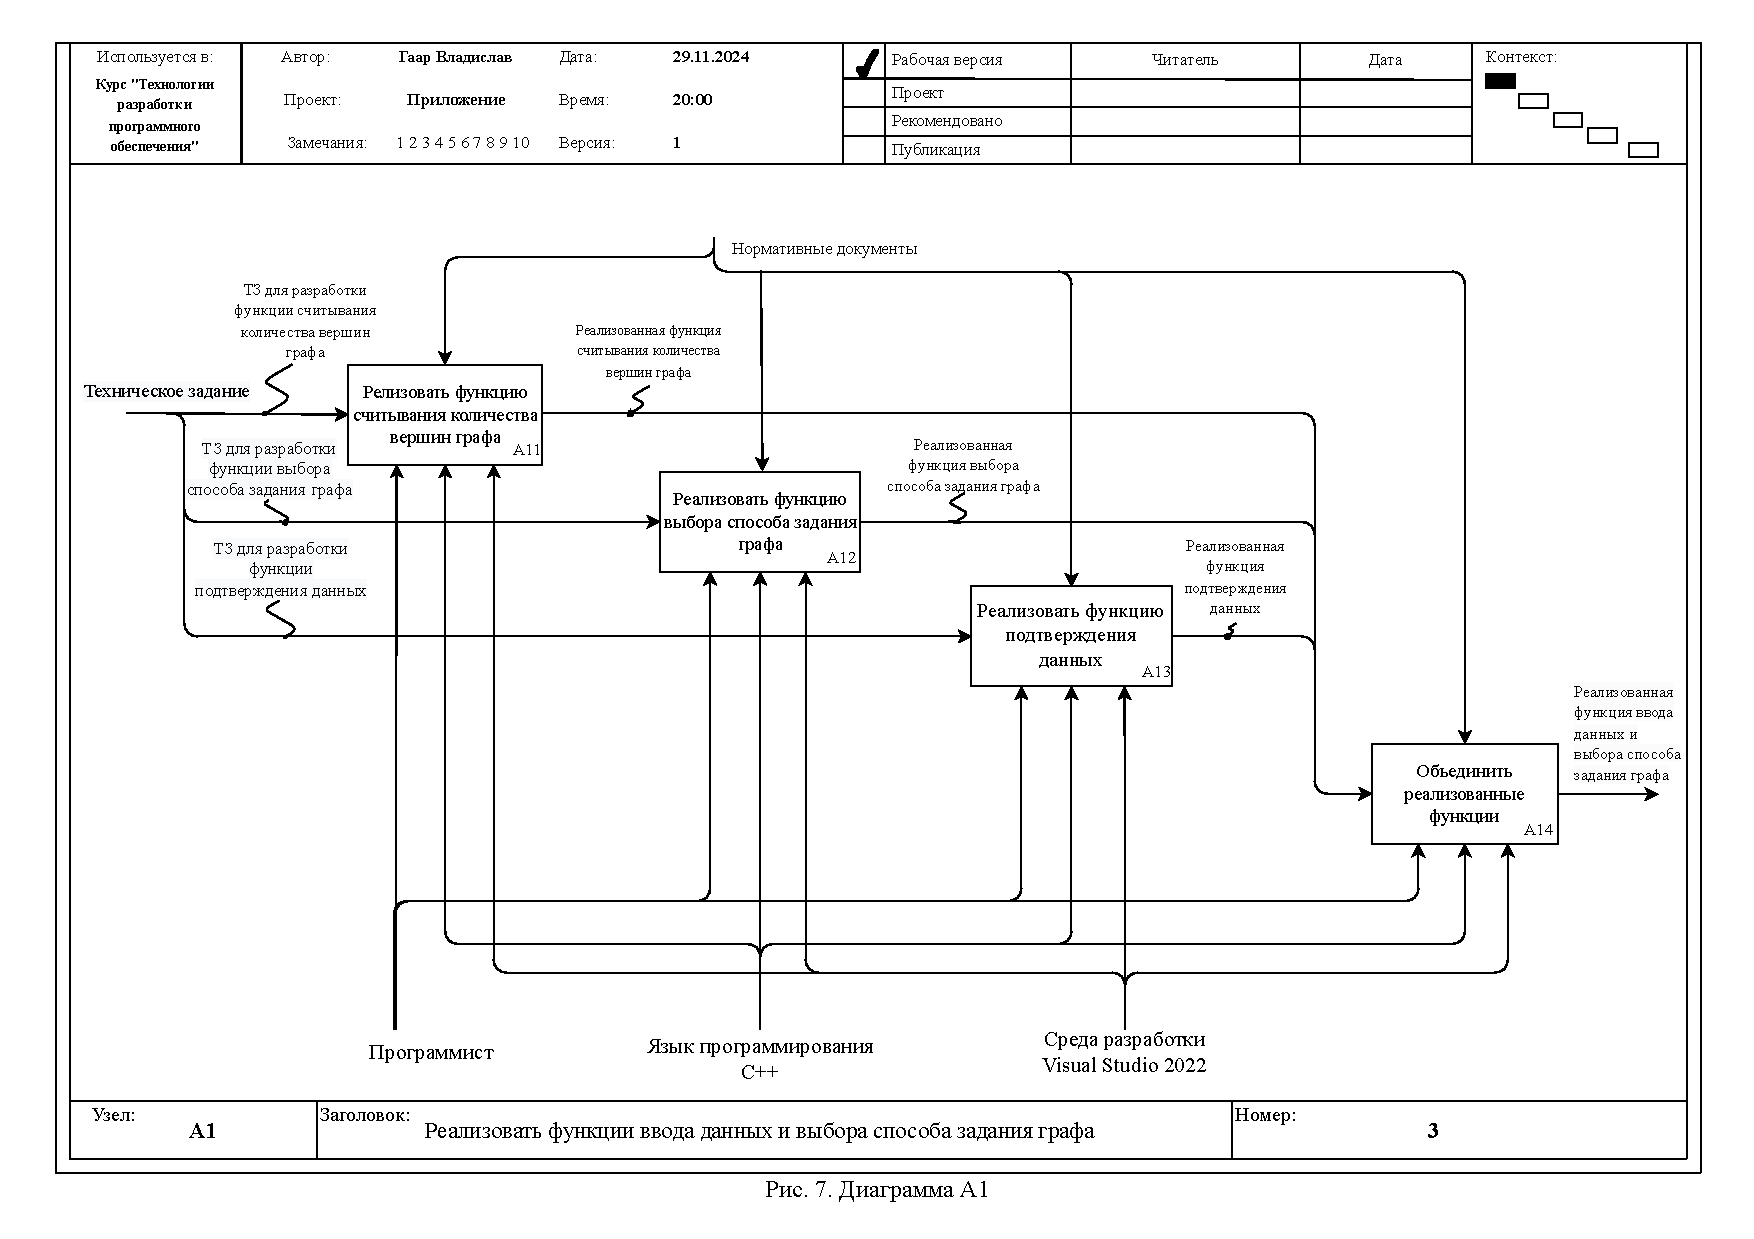
\includepdf[pages=1, fitpaper]{A1.pdf}


\subsubsection{Диаграмма А2}
На Рис. 4 представлено более подробное представление блока А2 <<Реализовать функцию генерации графа>>.

Диаграмма А2 является дочерней диаграммой для А0 (см. Рис. 1). Данная диаграмма представляет собой декомпозицию
блока реализации функции генерации графа на элементы, которые связаны между собой. 

Были выделены следующие блоки:
\begin{itemize}
	\item[A21.] Реализовать функцию генерации шаблона случайного графа
	\item[A22.] Релизовать функцию назначения весов рёбрам
	\item[A23.] Реализовать функцию проверки связности и ацикличности графа
	\item[A24.] Объединить реализованные функции
\end{itemize} 

\newpage
\hypertarget{img:A2}{}
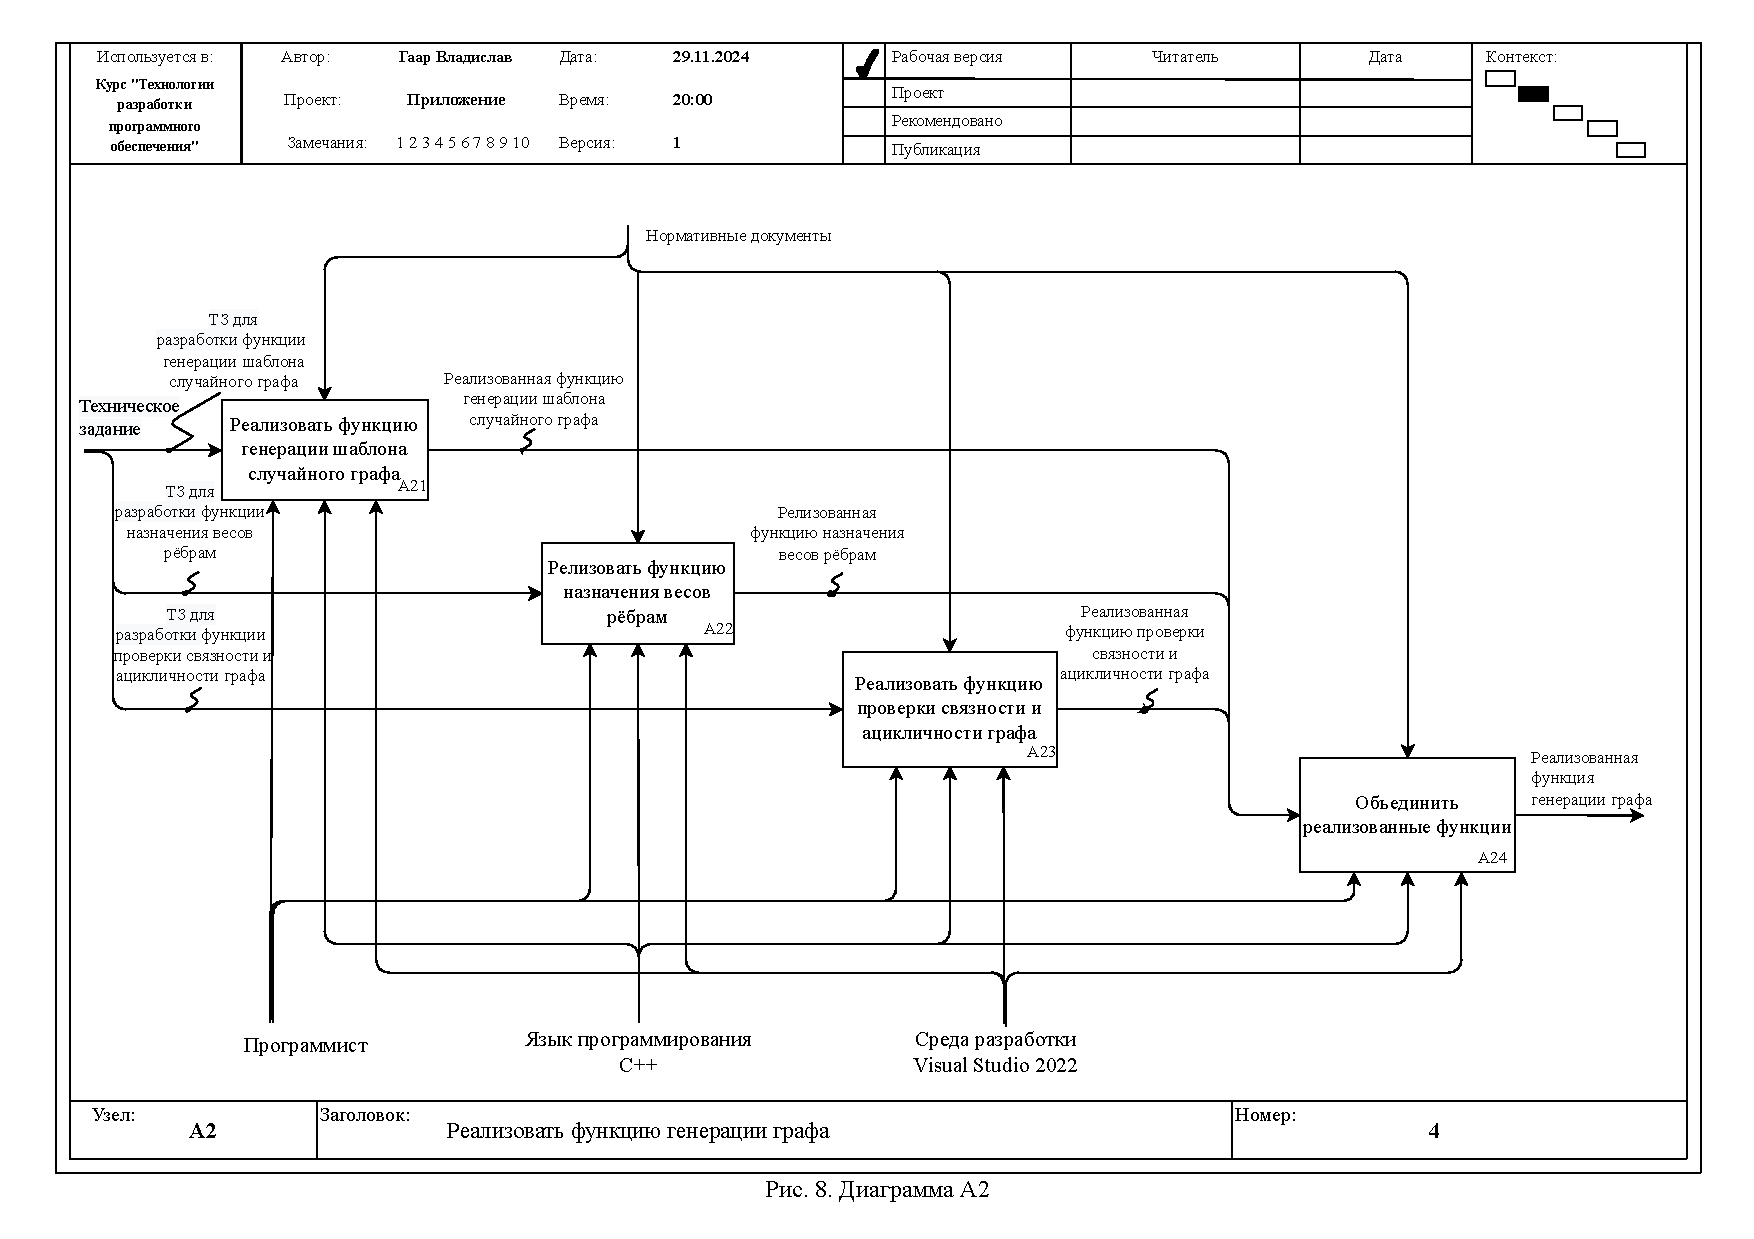
\includepdf[pages=1, fitpaper]{A2.pdf}


\cleardoublepage
\phantomsection
\newpage
\addcontentsline{toc}{section}{Заключение}
\section*{Заключение}
Таким образом, для разработки модели, демонстрирующей процесс создания модуля кодирования и декодирования графа кодом Прюфера,
была использована методология функционального моделирования IDEF0.

Благодаря данной методологии были выявлены и наглядно показаны основные этапы разработки приложения с точки зрения 
разработчика-программиста. Была построена контекстная диаграмма (родительская диаграмма), проведена ее декомпозиция и 
построены четыре дочерние диаграммы: А0, А1, А2. 

\cleardoublepage
\phantomsection
\newpage
%Список источников
\begin{thebibliography}{0}
	\bibitem{bib:gost_idef0}
	ГОССТАНДАРТ РОССИИ. Руководящий документ. МЕТОДОЛОГИЯ ФУНКЦИОНАЛЬНОГО МОДЕЛИРОВАНИЯ IDEF0. 
	Москва: ИПК Издательство стандартов, 2000г., 75с.

	\bibitem{bib:gost2_idef0}
	Методология IDEF0. Стандарт. Русская версия. МетаТехнология 1993, 91 с.
\end{thebibliography}
\addcontentsline{toc}{section}{Список источников}

\end{document}